\chapter{Studie}\label{Studie}
Um das System in der Praxis zu testen, musste im Anschluss eine Nutzerstudie durchgeführt werden.
Dies beinhaltete die Planung und Durchführung der Studie, sowie die Auswertung deren Ergebnisse.
Es musste der Rahmen der Studie geplant und Testpersonen angeworben werden, die darauf einen standardisierten Fragebogen ausfüllen und in einem Interview Fragen beantworten mussten.

\section{Entwurf}\label{Entwurf}
Nachdem die Umsetzung des Bauhausboards Systems abgeschlossen war, galt es einen Test mit Mitarbeitern der Medienfakultät der BUW durchzuführen.
\\
Dafür wurde am Uni-internen Rechenzentrum ein Linux Server mit 2,53GHz Intel Xeon Dualcore, 2GB RAM und Ubuntu Version 14.04 aufgesetzt.
Auf dem Server liefen Node.js, damit Bauhausboards ausgeführt werden konnte und Postfix\footurl{http://www.postfix.org} als Mailserver.
Dieser Mailserver konnte nur Emails an Adressen innerhalb des Universitätsnetzes verschicken, was für die Studie jedoch kein Problem darstellte.
\\
Als Displays wurden neue Tablets angeschafft, die mehr Leistung besaßen, als das Tablet aus der Vorstudie.
Es handelte sich dabei um vier Blaupunkt Discovery 1000c mit 10,1 Zoll Display, 1,33GHz AllWinner A33 Quadcore, 1GB RAM und Android\todotext{4.4 oder 5}. Mit vier Tablets konnten für die Studie vier Räume mit Displays ausgestattet werden.
\\
Damit die Benutzer, wie in der Vorstudie, nicht mit den vorinstallierten Applikationen der Tablets interagieren konnten, musste auch auf den neuen Tablets eine Kiosk-Applikation\footurl{http://www.android-kiosk.com} installiert werden.
\\
Zusätzlich zum Kiosk wurde eine Tasker-App\footurl{http://tasker.dinglisch.net} installiert.
Damit konnte man Aufgaben nach bestimmten Systemereignissen ausführen lassen.
Es wurde Task erstellt, der beim Start des Android-Systems automatisch die Kiosk-App startete, falls das System neu gestartet wurde.
\\
Als Diebstahlsicherung konnte man auf den Tablets Google Locate aktivieren.
Es diente zur Ortung der Geräte, falls diese gestohlen worden wären.
\\
\\
Um die Displays aufhängen zu können, musste eine geeignete Befestigungsmöglichkeit gefunden werden.
Jedoch sollten keine neuen Löcher zur Aufhängung an den Wänden neben den Büros entstehen.
Deswegen sollten die Displays erneut mit Hilfe der bereits aufgehängten Türschilder befestigt werden.
Da bei dieser Studie die Tablets nicht wie in der Vorstudie, durch Löcher in der Tablet-Rückwand, aufgehangen werden konnten, musste die Befestigung anders ausfallen.
Zu diesem Zweck wurden 3D gedruckte Eckstücke \abb{img:Eckstuecke}, mit denen die Tablets befestigt werden konnten, auf eine Plexiglasplatte geschraubt \abb{img:fertigeAufhaengung}.
Diese Aufhängung nutzte die Bohrlöcher für die bereits vorhandenen Türschilder mit, wodurch keinerlei Eingriff in die Bausubstanz entstand.
\\\todotext{Bild von den Eckstücken und von der fertigen Aufhängung}\\
\begin{figure}%[h!]
  \centering
    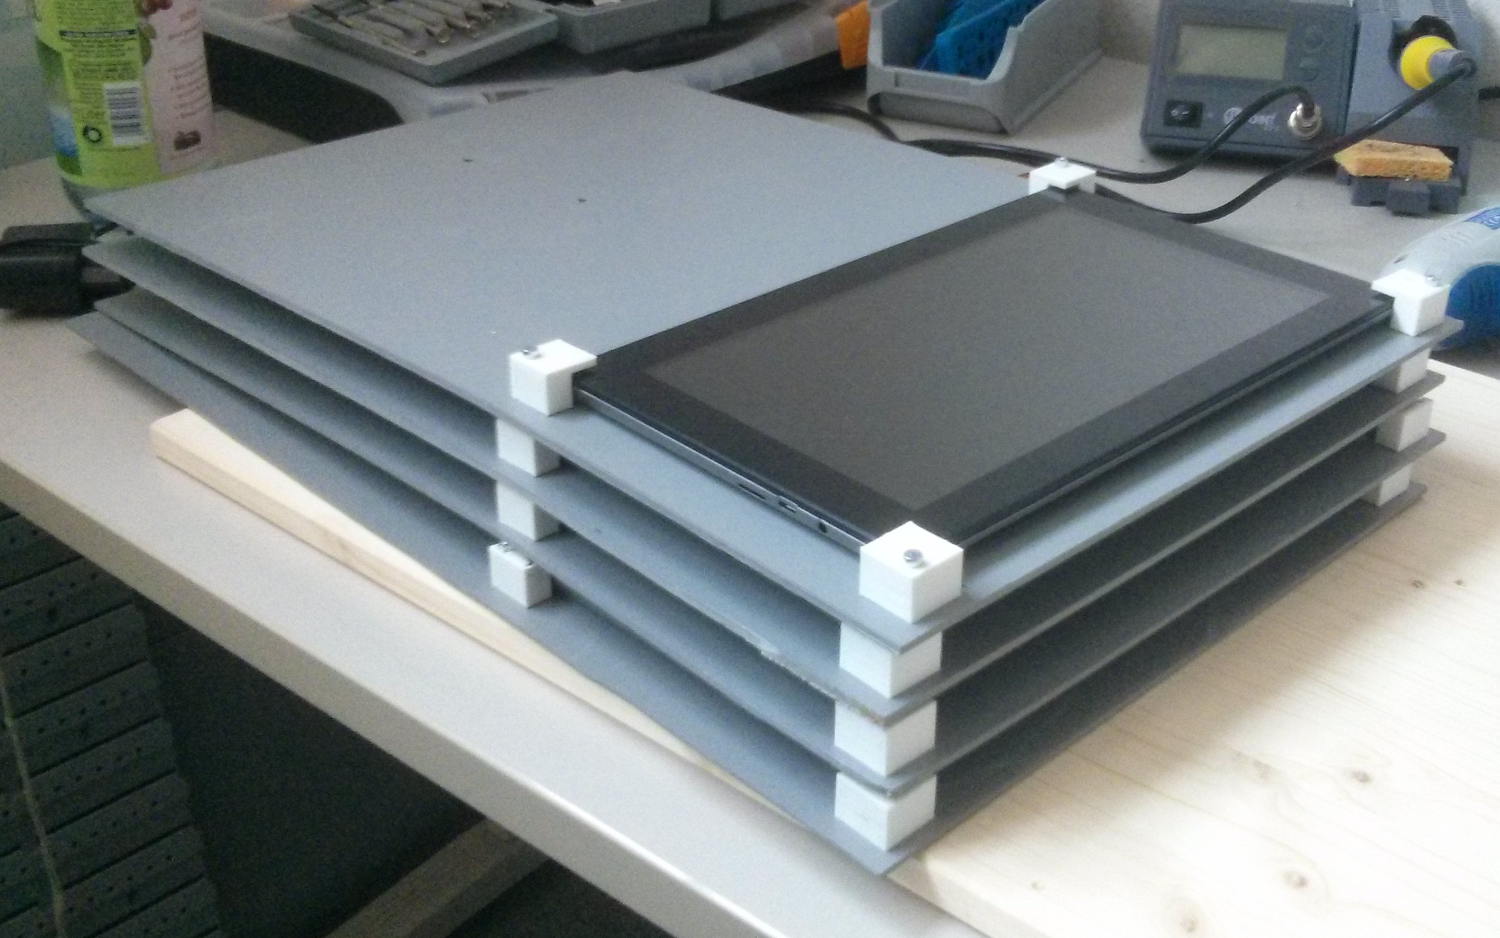
\includegraphics[width=0.85\textwidth]{./img/fertigeAufhaengung.png}
  \caption{Bauhausboards - Aufhängung}
  \label{img:fertigeAufhaengung}
\end{figure}
\\
Damit sich die Testnutzer mit der Grundlegenden Funktion von Bauhausboards vertraut machen konnten, habe ich ein Benutzerhandbuch erstellt.

% Nachdem Umsetzung abgeschlossen war: Test mit echten Nutzern
% Server mit NodeJS und Postfix aufgesetzt
% - Programm auf Server in Uni eingerichtet -> Spezifikationen? oder wurde das schon vorher angegeben?
% - Mailserver installiert, damit Server mails verschicken konnte (nur uni-intern)
% 4 Tablets angeschafft (Durch 4 Tablets -> 4 Räume zum Testen möglich)
%- Blaupunkt Discovery 1000c
%   * 10,1"
%   * CPU: Quadcore @ 1,33GHz
%   * Android 5.1
%   * 1GB RAM
%   * 1024x600 Auflösung (~17:10)
% Alle Tablets mit Kiosk-Mode Browser bestückt
%- Kiosk Mode Browser App auf Tablets um beenden der Bauhausboards App zu verhindern
%- Tasker zum automatischen start des kiosk modes nach systemstart - falls schlaue leute denken, sie können damit den kiosk browser umschiffen
%- Google Locate um Position des Tablets zu bestimmen, im falle eines Diebstahls
%- Rahmen: 4 Tablets -> 4 Räume
%- Wandbefestigung
%  * 3D gedruckte Eckstücke mit Loch um Tablets zu halten + zu sichern
%  * Holz/Blech Rückwand >> plexiglas
%  * Nutzung des vorhandenen Türschildes
%  * Fotos und 3D Model
%- Nutzer Tutorial zur Nutzung des Tools entworfen




\section{Durchführung}\label{Durchführung}
\todotext{Bild von aufgehängten Boards}\\

% Durchführung Studie in B11 BUW Medienfakultät
% 4 Räume im selben Gang
% ~10 Leute (2 CG Mitarbeiter + 7-8 VR Mitarbeiter)
% Alles Ph.D. oder angehende Ph.D.
% Tablets wurden vor deren Büros aufgehangen
% Einweisung der Testnutzer
% Durchlauf 2 Wochen 14Tage
% Zwischendurch ein zwei Fragen beantwortet
% Nach Studie:
%  * Ausfüllen UEQ Fragebogen (Was ist UEQ?)
%  * Interview mit allen Nutzern(mit Audiofile zur bessern Auswertung) zur Analyse der benutzten/nicht benutzten Funktionen








%- Bauhausstraße 11 Fakultät Medien
%- Da 4 Tablets 4 Räume für einen Testdurchlauf
%- Anzahl Tester in Räumen (10):
%  * 3 in VR1
%  * 3 in VR2
%  * 2 in VR3
%  * 2 in CG
%- Laufzeit 5Tage
%- UEQ Fragebogen nach Testlauf
%- Interview mit allen Testern
%  * FRAGEN ERSTELLEN
%- herausfinden wer so vorbeigehender Nutzer war
%  * Diese Leute gezielt ansprechen und auch mit Fragen löchern
%- Testpersonen das Frontend Testen lassen separat??
%- Aufnahme des Interviews (Audiofile)


\section{Auswertung}\label{Auswertung}
% Einfach die Ergebnisse der Studie und wie gut die Boards aufgenommen wurden

%- manche Nutzer haben nichtmal das Tutorial gelesen ...
% - Ein Großteil der Nutzer meinte, dass es unersichtlich ist, wer alles im Raum arbeite und es besser wäre, dass man auf den ersten Blick erkennen könnte, wer alles drin arbeitet (sowas wie Nutzerliste Rechts unter Header)
% - Ein Bug wurde entdeckt, dass wenn man noch keinen Content eingestellt hatte und man dann einen Hintergrund setzen will man ausgeloggt wird, da eine exception geschmissen wurde (Lösung eigene Background Tabelle in der DB)
% - Bei einem User ging nach einer weile der Sidebar nichtmehr (möglicherweise, weil js file nicht vollständig geladen und dadurch der swipe listener nicht feuerte)
% - Die UserImages sind manchmal verzerrt komischerweise